\documentclass[11pt,a4paper,bibliography=totocnumbered]{scrartcl}
\usepackage[utf8]{inputenc}
\usepackage[ngerman]{babel}
%\usepackage[USenglish]{babel}
\usepackage{booktabs}
\usepackage{braket}
\linespread{1.2}
\usepackage[T1]{fontenc}
\usepackage{amsmath,amssymb,amstext}
\usepackage{graphicx}
\usepackage{fancyhdr}
\usepackage{titling}
\usepackage{color}
\usepackage{array}
\usepackage{chemmacros}
\usepackage{float}
\usepackage{chemexec}     
\usepackage{chemfig,chemnum}
\usepackage{natbib} 
\usepackage[hyphens,spaces]{url}
\newcolumntype{M}[1]{>{\centering\arraybackslash}m{#1}}
\usepackage{multirow}
% URLs im pdf Dokument hinzufügen
\usepackage{hyperref}
\usepackage{sidecap}

\setlength{\parindent}{0em} 

\graphicspath{ {./picture/} }

\begin{document}
	
	\pagestyle{headings}
\pagenumbering{arabic} 

\section{Allgemein}

\subsection{stets im Hinterkopf behalten:}
\begin{enumerate}
\item die Formeln der Quantenmechanik sind häufig nur erraten
\item \textit{„vieles spricht dafür, dass der Zufall eine fundamentale Rolle in der Natur spielen könnte und dass 
das Teilchen vor der Ortsmessung gewissermaßen selbst noch nicht weiß, wo es sich materialisieren soll.“} \\
$\rightarrow$ hier: \textbf{Wahrscheinlichkeitsinterpretation}
\item eine Wellenfunktion \underline{muss} bei der Wahrscheinlichkeitsinterpretation normiert sein (\ref{normiert})
\item physikalisches System kann nur \textbf{diskrete Werte} der Energien (z.B. Drehimpuls) annehmen
\end{enumerate}

\subsection{Postulate:}
\begin{enumerate}
\item $\psi(\vec{r}_1,\vec{r}_2, ...,\vec{r}_N,t)$ ist unser Zustand/Eigenfunktion des Teichensystem (Anzahl $N$ Teilchen), mit den Ortsvektoren $\vec{r}$
\item \textbf{gilt universell:} jede physikalisch messbare Variable besitzt einen hermitischen Operator ($\hat{A}$, $\hat{B}$, ...) (\ref{Operatoren}).\\
 if $[\hat{A},\hat{B}]=0$:
\begin{enumerate}
    \item $\hat{A}$ und $\hat{B}$ sind hintereinander messbar
    \item $\hat{A}\ket{\psi}=\lambda\ket{\psi}$ und $\hat{B}\ket{\psi}=\mu\ket{\psi}$
\end{enumerate}
\item nur die Eigenwerte ($\lambda,\mu$ etc.) sind messbar; sie sind reelle Zahlen 

\end{enumerate}



\subsection{Unterschiede Quantenmechanik (QM) zur Elektrodynamik (ED):}
\begin{enumerate}
    \item ED: \textbf{Felder} (z.B. $\vec{B}$) sind die physikalische Rolle:
    \begin{enumerate}
        \item deren Werte bestimmen an jedem Ort, welche Kraft auf die Ladung $q$ wirkt

    \end{enumerate}
    \item QM: \textbf{Potentiale} sind die physikalische Rolle
\begin{enumerate}
    \item z.B. das \textcolor{red}{Vektorpotential} $A$ von $\vec{B}$ beeinflusst die Phase einer Quantenwelle 
\end{enumerate}
\end{enumerate}

\newpage
	\section{Die statistische Quantenwelle $\psi$}

\subsection{zum Verständnis:}
\begin{enumerate}
    \item die Wahrscheinlickeitsaussagen sind die Lösung der Schrödinger-Gleichung (\ref{schroedinger})
    \item ein $e^-$ hat in einem Atom keine Flugbahn. $\psi$ der $e^-$ sagt nur wie wahrscheinlich es ist,
    irgendwo ein $e^-$  anzutreffen, wenn man es experimentell misst
    \item durch Messung \textit{kollabiert} $\psi$ zu einem Peak am gemessenen Wert 
    \item es gilt die Heisenberg'sche Unschärferelation $\sigma_x\sigma_p\geq\frac{\hbar}{2}$ (siehe \ref{Varianz})
\end{enumerate}

\subsection{Bedingungen aus der Statistik:}
\begin{enumerate}
    \item allgemein: $\braket{\psi_m|\psi_n}=\int \psi_m^*\psi_n \,dr=\int_{-\infty}^{\infty}\rho(r)\,dr=\delta_{mn}$ 
    mit Wahrscheinlichkeitsdichte $\rho(r,t)=|\psi(r,t)|^2$
    \item da $\int_{-\infty}^{\infty} \rho(r) \,dr=1$ muss $\psi$ normiert sein, damit 
    das Teilchen nicht zu einer Wahrscheinlichkeit ungleich 100 $\%$ im ganzen Raum vorfindbar ist \label{normiert}
    \item Erwartungswert/Mittelwert $\bar{A}\equiv\braket{A}=\braket{\psi|\hat{A}\psi}=\int_{-\infty}^{\infty}\hat{A}\rho(r)\,dr$
    \item Varianz $\sigma^2=\braket{A^2}-\braket{A}^2$ \label{Varianz}
\end{enumerate}

\subsection{Schrödinger-Gleichung:}\label{schroedinger}
\begin{enumerate}
    \item die Schrödinger-Gleichung hängt nur von zwei Funktionen ab: $\psi$ und Potential $V$\\
    $\rightarrow$ \textbf{Hinweis:} Auswahl Koordinatensystem durch $\Delta$ 
    \item (allg.) zeitabhängige: $i\hbar\frac{\partial\psi\left(x,t\right)}{\partial t}=-\frac{\hbar^{2}}{2m} \Delta \psi\left(x,t\right)+V\cdot\psi\left(x,t\right)=\hat{H}\psi\left(x,t\right)$
    \begin{enumerate}
        \item \textbf{Separationsansatz} (um Funktionen aufzuteilen): $\psi(x,t)=\varphi(x)\cdot f(t)$
    \end{enumerate}


    \item zeitunabhängige: $-\frac{\hbar^{2}}{2m}\Delta\psi\left(x\right)+V(x)\cdot\psi\left(x\right)=E\psi\left(x\right)$ 
    \begin{enumerate}
        \item auch geschrieben als $\hat{H}\psi=E\psi$
    \end{enumerate}
\end{enumerate}
\newpage

\subsection{Modellsysteme für die Form des Potentials $V$:}
\begin{enumerate}
    \item freies Teilchen (d.h. $V=0$):
    \begin{enumerate}
        \item zeitabhängiges Teilchen ist eine ebene Welle ($\psi$ kann zum Zeitpunkt $t=0$ 'lokalisiert'  
        und dort \textbf{normiert} werden) \\
        $\rightarrow$ $\psi =Ae^{i(kx-\omega t)}$ mit $\omega=\frac{E}{\hbar}$
        \item die Geschwindigkeit ist durch die Gruppengeschwindigkeit $v_g=\frac{\hbar k}{m}=\frac{d}{dk}\omega$ und \underline{nicht}
        durch die Phasengeschwindigkeit von $\psi$ gegeben
        \item \textbf{Model vom unendlichen Potentialtopf anwendbar}
    \end{enumerate}
    \item unendlicher Potentialtopf ($V(x)=0$ für $0\leq x\leq L$, sonst $V(x)=\infty$)
        \begin{enumerate}
            \item $\psi(x)=A\sin(\frac{n\pi x}{L})$
            \item $E_n=\frac{n^2 \pi^2 \hbar^2}{2mL^2}$ mit $L$: Länge des Topfes 
            \item \textbf{Anwendung} in der Berechnung von Absorptionsenergien ($\Delta E$: HOMO $\rightarrow$ LUMO) bei Molekülorbitalen 
        \end{enumerate} 
    \item harmonischer Oszillator ($V=\frac{1}{2}m\omega^2x^2$):
    \begin{enumerate}
        \item $E_n=\hbar\omega(n+\frac{1}{2})$ mit $n=0,1,2,...$
        \item 2 Lösungsansätze (mit Quantenzahl $n$):
        \begin{enumerate}
            \item $\psi_n(x)=$ Normierung * (Polynom in x) * (Gauß-Funktion)\\
            $\rightarrow$ $\psi_n(x)=A_n\cdot H_n(x) \cdot e^{-0.5x^2}$ \\
            die Lösungen davon sind die Hermite-Polynom $H_n(x)$, die man nachschlagen kann
            \item Leiteroperatoren $\hat{a}_\pm$ verringern/erhöhen die Energien einer bekannten Lösung in diskrete Schritte:\\
            $\hat{H}\psi=\hbar \omega(\hat{a}_\pm \hat{a}_\mp \pm 0.5)\psi=E\psi$ , mit $\hat{a}_\pm=\frac{1}{\sqrt{2\hbar m \omega}}(\mp i\hat{p}+m \omega\hat{x})$ \\
            \underline{Hinweise}:
            \begin{enumerate}
                \item $\hat{a}_\pm$ wird direkt auf $\psi$ angewendet 
                \item $\hat{a}_- \psi_0=0$, da man vom untersten Energieniveau nicht 'absteigen' kann
            \end{enumerate} 
            $\rightarrow$ $\psi_n(x)=A_n\cdot (\hat{a}_+)^n \cdot \psi_0(x)$
        \end{enumerate}

    \end{enumerate}
    \item Potentialstufe ($V(x)=V_0$ für $0\leq x$, sonst $V(x)=0$)
    \begin{enumerate}
        \item Fallunterscheidung, ob $E>V_0$ oder $E<V_0$
    \end{enumerate}
    \item Potentialbarriere ($V(x)=V_0$ für $-a\leq x \leq +a$, sonst $V(x)=0$; mit Breite $2a$) \label{Potentialbarriere}
\end{enumerate}




\newpage
	\section{Arbeiten mit $\psi$}

\subsection{Grundregeln für Verwendung von $\psi$:}
\begin{enumerate}
    \item die Energieniveaus spalten sich im homogenen $\vec{B}$ auf: Zeeman-Effekt genannt
    \item klassisch erlaubt: $V<E$ $\rightarrow$ "oszillierendes Verhalten von $\psi$"
    \item klassisch verboten: $V>E$ $\rightarrow$ Tunneleffekt kann auftreten (u.a. bei einer \textbf{Potentialbarriere} (\ref{Potentialbarriere}))
    \item $\psi$ besitzt Quantenzahlen: $n$ bestimmt $l$, $l$ bestimmt $m$
    \begin{enumerate}
        \item Quantenzahl $n$ (legt die diskreten Energiestufen fest): $n=1,2,3,...$
        \item Bahnquantenzahl $l$ (gehört zu $L^2$): $0\leq l\leq n-1$ (\textbf{Anmerkung}: können nur ganzzahlig oder halbzahlig sein)
        \item magnetische Quantenzahl $m$ (gehört zu $L_z$): $m=-l,...,+l$ (\textbf{Anmerkung}: in ganzzahligen Schritten)
    \end{enumerate}
\end{enumerate}

\subsection{Photonen:}
\begin{enumerate}
    \item Wellenpackete $=$ Überlagerung von ebenen Wellen
\end{enumerate}

\subsection{Messung von $\psi$ mittels hermitische Operatoren:} \label{Operatoren}
\begin{enumerate}
    \item Ort: $\hat{x}$
    \item Impuls: $\hat{p}$
    \item Gesamtenergie: $\hat{H}$
    \item Drehimpuls: $\hat{L}_i=\sum_{jik}\epsilon_{ijk}\hat{x}_j\hat{p}_k$ (\ref{Drehimpuls})
    \begin{enumerate}
        \item "Betragsinformation": $\hat{L}^2$
        \item (teilweise) "Richtungsinformation": $\hat{L}_z$
    \end{enumerate}

\end{enumerate}

\subsection{die 2 Drehimpulse $L$ (\textbf{Einheit}: [$\hbar$]):} \label{Drehimpuls}
\begin{enumerate}
    \item nice to know:
    \begin{enumerate}
        \item die Eigenwerte von $\hat{L}^2$ sind $\lambda=\hbar^2 l (l+1)$
        \item die Eigenwerte von $\hat{L}_z$ sind $\lambda=\hbar m$, mit Quantenzahl $m$
        \item $[\hat{L}^2,\hat{L}_z]=0$
        \item $\hat{L}_\pm=\hat{L}_x \pm i\hat{L}_y$
        \begin{enumerate}
            \item $\hat{L}_\pm$ verändert den Eigenwert von $\hat{L}_z$ um $\pm \hbar$, was die Einheit des Drehimpuls entspricht!
            \item $\hat{L}_\pm$ verändert \underline{nicht} den Eigenwert von $\hat{L}^2$
        \end{enumerate}
    \end{enumerate}
    \item Bahndrehimpuls:
    \begin{enumerate}
        \item nimmt nur ganzzahlige Werte für $l$ ein: $l=0,1,2,3,...$
        \begin{enumerate}
            \item $l=0\rightarrow$ s-Orbitale
            \item $l=1\rightarrow$ p-Orbitale
            \item $l=2\rightarrow$ d-Orbitale
        \end{enumerate}
    \end{enumerate}
    \item Spin $s$: eine Art ewige Eigendrehung der Teilchen
\begin{enumerate}
    \item aus dem Spin-Statistik-Theorem:
\begin{enumerate}
    \item Fermionen (z.B. $e^-$, Proton, Neutron): s=0.5  $\rightarrow$ $\psi$ ist antisymmetrisch
    \begin{enumerate}
        \item Fermionen sind „Einzelgänger“ d.h. sie können nicht am selben Ort sein
    \end{enumerate}
    \item Bosonen (z.B. Photonen): s=1 $\rightarrow$ $\psi$ ist symmetrisch 
    \begin{enumerate}
        \item Bosonen sind „Herdentiere“ (lieben Gleichschritt) d.h. z.B.  können sich unzählige
        Photonen zusammentun und gemeinsam eine schwingende elektromagnetische Welle ausbilden 
    \end{enumerate}
\end{enumerate}
\item $s=0.5$:
\begin{enumerate}
    \item $s=0.5$ $\rightarrow$ $m_s=-0.5$ und $m_s=+0.5$
\end{enumerate}
\end{enumerate}
\end{enumerate}



\subsection{Störung des System (Störungstheorie):}
\begin{enumerate}
    \item Grundannahmen:
    \begin{enumerate}
        \item die Lösung des ungestörten System ist bekannt
        \item die Störung ist klein
    \end{enumerate}
\end{enumerate}
	\section{Näherungsmethoden zum Lösen der Schrödinger-Gleichung von nicht-idealisierten Systemen}
\subsection{Störungstheorie (Störung des System):}
\begin{enumerate}
    \item Grundannahmen:
    \begin{enumerate}
        \item die Lösung des ungestörten System $\psi^\textbf{0}$ (die '0' kenntzeichnet das ungestörte System) ist bekannt
        \item die Störung ist klein
    \end{enumerate}
    \item Folgen:
    \begin{enumerate}
        \item die Störung führt allgemein zur Aufhebung der Entartung 
    \end{enumerate}
\end{enumerate} 

\subsection{Variationsprinzip}
\begin{enumerate}
    \item Grundgedanke: Grundzustandenergie $E_0$ berechnen wollen
    \begin{enumerate}
        \item eine obere Schranke für $E_0$ wird durch Hilfe einer Test-Wellenfunktion errechnet, die wir dann durch Minimierung 
        (Optimierungsprozess somit) möglichst nah in Richtung des exakten Wertes herunterrechnen.
    \end{enumerate}
\end{enumerate}

\subsection{Born-Oppenheimer Näherung (Adiabatische Näherung)}
\begin{enumerate}
    \item Anwendung: \textbf{Moleküle}
    \item Grundgedanke: Separation des Problems in schnelle $e^-$ und langsame Kerne
\end{enumerate}

\newpage
	\section{Simulation (z.B. Molekülsimulation (molecular dynamic) für die Pharma Industrie) mittels eines Quantencomputer}

\begin{enumerate}
    \item die Quantenwelle $\psi$ 'bewegt' sich (wir wissen nicht, wo $\psi$ liegt) im Raum (Abb. \ref{bloch}) und hat den Zustand $\ket{\psi}$
        (als Vektor/Pfeil dargestellt)
    \begin{SCfigure}[][h!]
        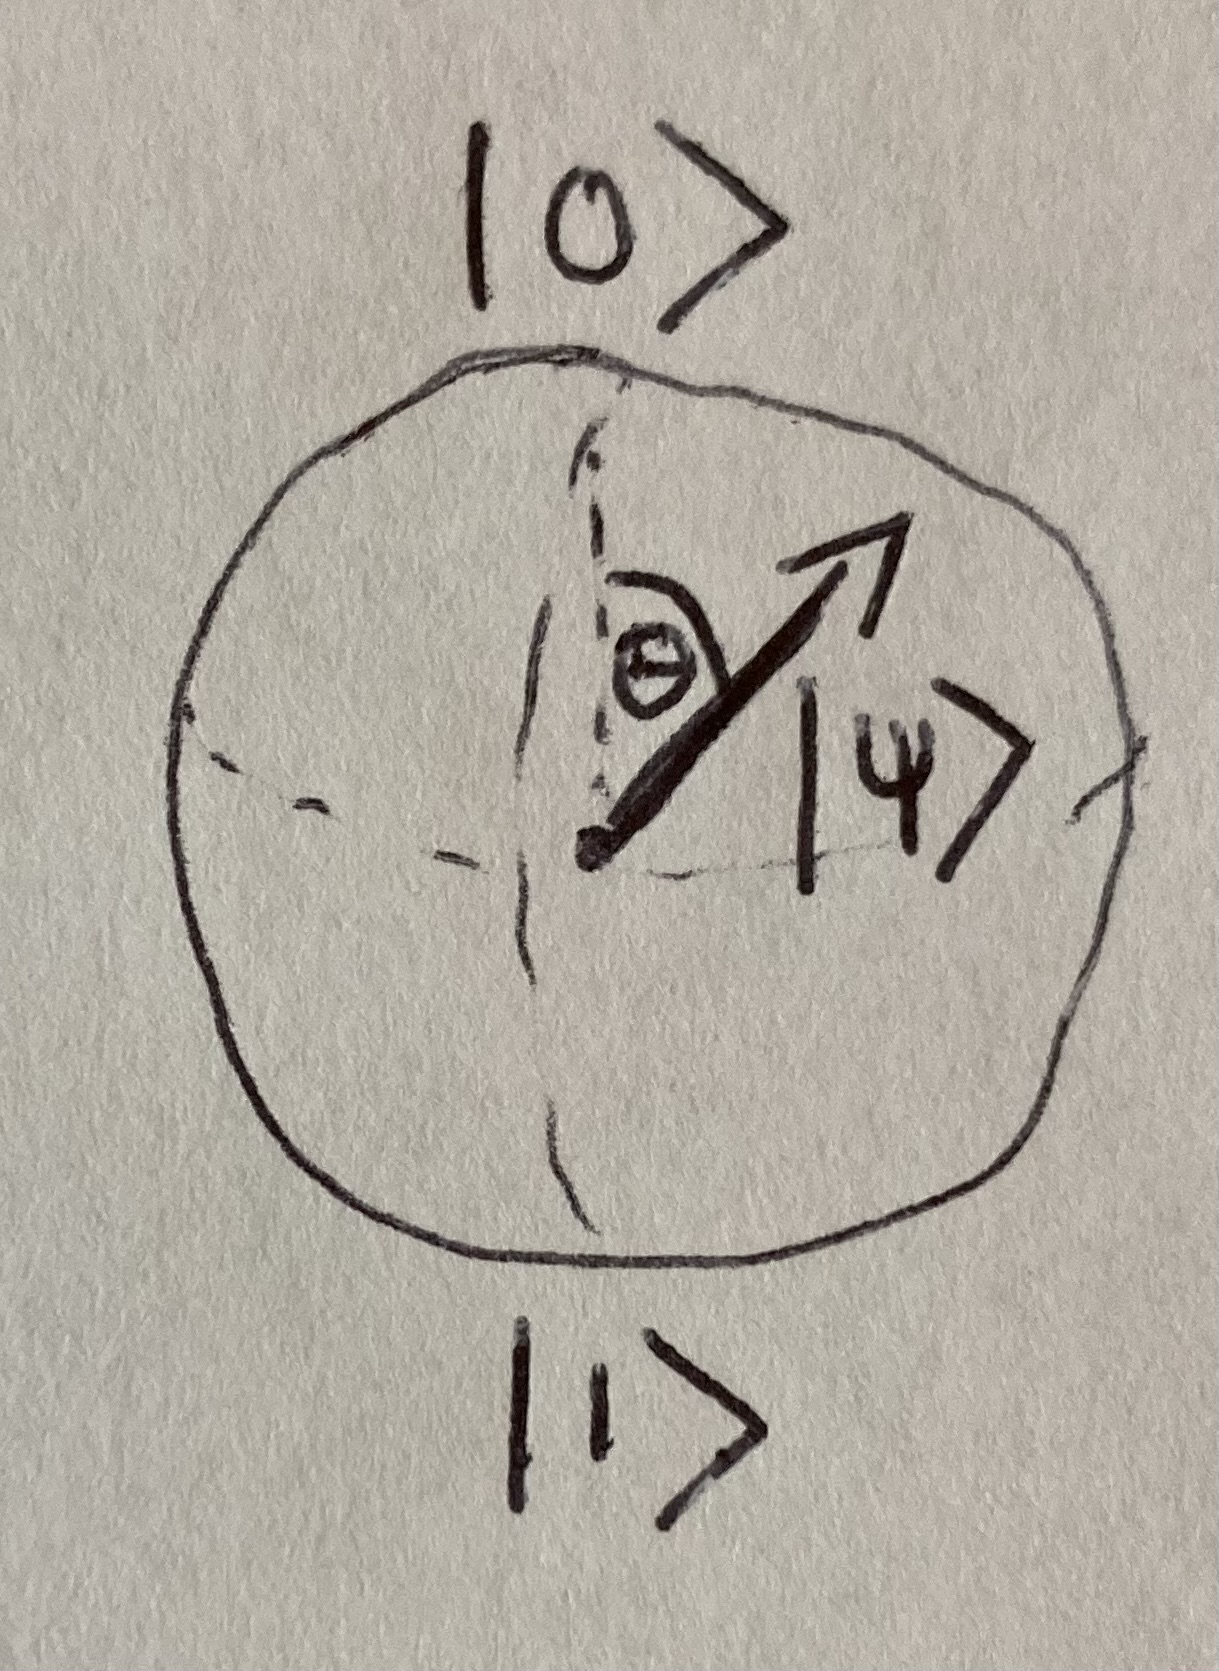
\includegraphics[width=0.35\textwidth]{bloch_kugel.png}
        \caption{Bloch-Kugel (zur Visualisierung eines 2 Zustände ($\ket{0}$ oder $\ket{1}$) Qubit), auf der
                    alle Zustände von $\ket{\psi}$ durch Punkte auf der Kugel Oberfläche beschrieben werden} 
        \label{bloch} 
    \end{SCfigure}
    \item Wir versuchen mathematisch eine Aussage zu machen, wie wahrscheinlich (Wahrscheinlichkeitsverteilung P(x) (Statistik)) es ist, dass $\ket{0}$
        oder $\ket{1}$ eintritt (z.B. P($\ket{0})$=0.7)):
        \begin{equation*}
            \psi(\vec{x})=\braket{\vec{x}|\psi}
        \end{equation*}
        mit $\ket{\vec{x}}=\ket{0}$ oder $\ket{1}$ (siehe Bloch-Kugel)
    \item Da sich die Quantenwelle 'bewegt', liegen die Zustände $\ket{0}$ und $\ket{1}$ $\underline{vor}$ der Messung
        in Superposition vor (\textbf{Gedankenexperiment}: Schrödinger Katze). Diese Superposition ist eine Teil der Kohärenzeigenschaft, worunter 
        die Überlagerung von Wellen und Teilchen Eigenschaft, sowie die Verschränkung auch fällt. Kohärenz und die damit 
        verbundene Zeitdauer (=Kohärenzzeit) erlaubt das Auftreten von quantenmechanischen Effekten und damit auch 
        die quantenmechanischen Berechnungen.
        \begin{equation*}
            \ket{\psi}=a\ket{0}+b\ket{1} 
        \end{equation*}
        (mit $\vert a\vert^2+\vert b\vert^2=1$)\\
        \underline{hier}:
        \begin{equation*}
            \ket{\psi}=\cos(0.5\theta)\ket{0}+e^{i\psi}\sin(0.5\theta)\ket{1}
        \end{equation*}
    \item Sobald wir messen, kollabiert $\psi$ auf einen messbaren Zustand ($\ket{0}$ oder $\ket{1}$) (seinen 'Eigenwert' $\lambda$). Die Superposition
        wird dabei zerstört, was eine Aufhebung der Köhrenz und damit verbundenes Ende der Quanteneffekte darstellt. Zusätzlich 
        kann die Superposition auch durch Wechselwirkung mit der Umgebung ungewollt zerstört werden.
    \item Beim Quantencomputer kann man $\underline{vor}$ der Messung (welche durch einen hermitischen Operator $\hat{A}, \hat{H}$ etc. erfolgt)
        den Zustand $\ket{\psi}$ durch Einsatz von Quantengatter noch ändern. Dies passiert durch Pulse von Mikrowellen auf den Qubit. 
        Quantengatter sind z.B.:
        \begin{enumerate}
            \item NOT Gatter
            \item Haddamard Gatter 
            \item Phasen Gatter
        \end{enumerate}
        Schaltet man mehrere Quantengatter hintereinander, bildet das den Quantenalgorithms, welcher oft auch quantum circuit
        bezeichnet wird. Dies ist momentan wie eine 'black box'. Die Algorithmen werden nach einen Trial and Error Prinzip entworfen,
        da man ja vorher nicht weiß, welche Lösung für das gestellte Problem die Richtige ist. Dies ist wie bei den Formeln der Quantenmechanik, 
        welche häufig auch nur erraten sind. Die Grundlage der Wirklichkeit ist nicht bekannt. Vlt. werden deshalb auch die Entwicklung von
        Quantenalgorithmen immer eine 'black box' bleiben. 
\end{enumerate}
Abschließend möchte ich noch sagen, dass beim Doppelspalt-Versuch wir auch die Atome/Moleküle nur mit ihren jeweiligen 
kohärenten Zustand $\ket{\psi}$ auf den Bildschirmdetektor schießen.\\
Die Kohärenzzeit muss erhöht werden, damit das Quantenverhalten nicht so schnell verloren geht.





\end{document}